% =========================================================================== %

\begin{frame}[t,plain]
\titlepage
\end{frame}

% =========================================================================== %

\begin{frame}{C++ -- Eine mächtige Sprache}
%
\begin{warnbox}
C++ ist eine eigenständige Sprache! Trotz großer Ähnlichkeiten sollten die beiden nie \enquote{unter einen Hut gesteckt} werden.
\end{warnbox}
%
\begin{itemize}
\item Formell: Weiterentwicklung von C -- vgl. Inkrement-Operator
\item Eigener Compiler \texttt{g++} ersetzt \texttt{gcc}.
\item \texttt{gcc} und \texttt{g++} für beide Sprachen geeignet, jedoch unterschiedlich optimiert
\item Viele neue Konzepte, von denen hier nur einige exemplarisch gezeigt werden
\item \emph{Gigantische} Sammlung von Routinen in der Standard-Library (STL)
\item Support: \url{http://en.cppreference.com} bzw. \url{http://de.cppreference.com}
\item UR bietet eigenen Kurs an:
	\href{http://www.physik.uni-regensburg.de/studium/it/c++kurs/}
	{$\rightarrow$ Programmieren mit C++ und der Qt-Bibliothek $\leftarrow$}
\end{itemize}
%
\end{frame}

% =========================================================================== %

\begin{frame}[fragile]{C vs. C++ -- Unterschiede}
%
\begin{columns}[T]
\column{.5\linewidth}
\begin{itemize}
\item Stream-Konzepte
	\begin{itemize}
	\item Bereitstellung eines Puffers
	\item User schreibt in Puffer
	\item System gibt gepufferete Daten zu geeigneter Zeit an Geräte wie Bildschirm weiter
	\item \texttt{printf} $\rightarrow$ \texttt{cout}
	\item \texttt{scanf}  $\rightarrow$ \texttt{cin}
	\end{itemize}
\item Function Overloading
\item Namespaces
\item Klassen -- Objektorientierung
\item Templates
\end{itemize}
%
\column{.5\linewidth}
\begin{codebox}[Beispiel: Hello World in C++]
\begin{minted}[fontsize=\scriptsize, linenos]{c++}
#include <iostream>

using namespace std;

int main (void) {
  int a, b, c;
  
  cout << "Hello world" << endl;
  cout << "Please enter 3 ints:" << endl;
  cin  >> a >> b >> c;
  cout << "You entered:" << endl;
  cout << a << b << b << endl;
  return 0;
}
\end{minted}
\end{codebox}
\end{columns}
%
\end{frame}

% =========================================================================== %

\begin{frame}[fragile]{Default Arguments und Function Overloading}
%
\vspace{-6pt}
\begin{columns}[T]
\column{.5\linewidth}
\begin{itemize}
\item Default Arguments
	\begin{itemize}
	\item Parameter beim Aufruf \enquote{auslassbar}
	\item Wenn ausgelassen: Zuweisung von Default-Wert
	\end{itemize}
\item Function Overloading
	\begin{itemize}
	\item Mehrere Funktionen mit gleichem Namen
	\item Aber: Unterschiedliche Art und/oder Anzahl von Parametern
	\item Zweck: Selbe Aufgabe für unterschiedliche Parametertypen oder Rückgabetypen erfüllen
	\item Code der einzelnen Funktionen unabhängig
	\end{itemize}

\end{itemize}
\column{.5\linewidth}
\vspace{-6pt}
\begin{codebox}[Beispiel: Default Arguments]
\begin{minted}[fontsize=\scriptsize, linenos]{c++}
int getBiggestIdx(
   int * arr, int N, 
   int first=0, int last=-1);
...
cout << getBiggestIdx(arr1, N, 5);
cout << getBiggestIdx(arr2, N,  , 7);
\end{minted}
\end{codebox}
%
\vspace{-12pt}
\begin{codebox}[Beispiel: Function Overloading]
\begin{minted}[fontsize=\scriptsize, linenos]{c++}
double distance(double x1, double y1,
                double x2, double y2);

double distance(double x1, double y1, 
                double z1,
                double x2, double y2, 
                double z2);
\end{minted}
\end{codebox}
\end{columns}
%
\end{frame}

% =========================================================================== %

\begin{frame}[fragile]{Strings in C++}
%
\begin{columns}[T]
\column{.5\linewidth}
\begin{itemize}
\item Eigener \enquote{Datentyp} (eigentlich: \emph{Klasse})
\item Baut auf C-String auf
\item Kommt mit einer großen Zahl von \emph{Methoden}: Routinen, die auf Strings angewandt werden können
\item STL-Header \texttt{string}
\item \texttt{at} -- Elemente lesen oder schreiben mit \emph{boundary check}
\item \texttt{size}, \texttt{length} -- Zeichen bis zum ersten \texttt{NULL}-Char
\item \texttt{capacity} -- Größe des zugrunde liegenden \mintinline{c}{char}-Arrays
\end{itemize}
%
\column{.5\linewidth}
\vspace{-12pt}
\begin{codebox}[Beispiel: Hello World in C++]
\begin{minted}[fontsize=\scriptsize, linenos]{c++}
#include <iostream>
#include <string>
using namespace std;

int main (void) {
  string myStr = "some funky words";
  
  // output entire string
  cout << myStr << endl;
  
  // output 4th char -- boundary check
  cout << myStr.at(3);  // or myStr[3]
  
  // change 9th char
  myStr.at(8) = 'n'
  return 0;
}
\end{minted}
\end{codebox}
\end{columns}
%
\end{frame}

% =========================================================================== %

\begin{frame}[fragile]{Strings in C++ (Fortsetzung)}
%
\begin{columns}[T]
\column{.45\linewidth}
\begin{itemize}
\item \texttt{clear} -- String leeren
\item \texttt{insert(where, count, what)} -- Anderen String einfügen
\item \texttt{find\_first\_of(what)} -- Zeichen in einem String finden
\item und viele mehr
\item[\Thus] \url{http://en.cppreference.com/w/cpp/string/basic_string}
\end{itemize}
%
\column{.55\linewidth}
\vspace{-12pt}
\begin{codebox}[Beispiel: Insert Strings]
\begin{minted}[fontsize=\scriptsize, linenos]{c++}
#include <iostream>
using namespace std;

int main (void) {
  string s = "something Hieronymus";
  
  s.insert(
    s.find_first_of(' ') + 1,
    "funny about "
  );
  
  cout << s;
  
  return 0;
}
\end{minted}
\end{codebox}
\end{columns}
%
\end{frame}

% =========================================================================== %

\begin{frame}{Warum immer noch C lernen?}
%
\tcbset{width=.495\linewidth, on line}
%
\begin{tcolorbox}[title=Zitat, height=4cm]
%
\vspace{5pt}
\begin{quotation}
In C++ it’s harder to shoot yourself in the foot, but when you do, you blow off your whole leg.
\end{quotation}
\vspace{-11pt}
%
\begin{flushright}
\footnotesize \href{https://www.youtube.com/watch?v=9QKHg8wj4MA}{Bjarne Stroustrup, Entwickler von C++}
\end{flushright}
%
\end{tcolorbox}
%
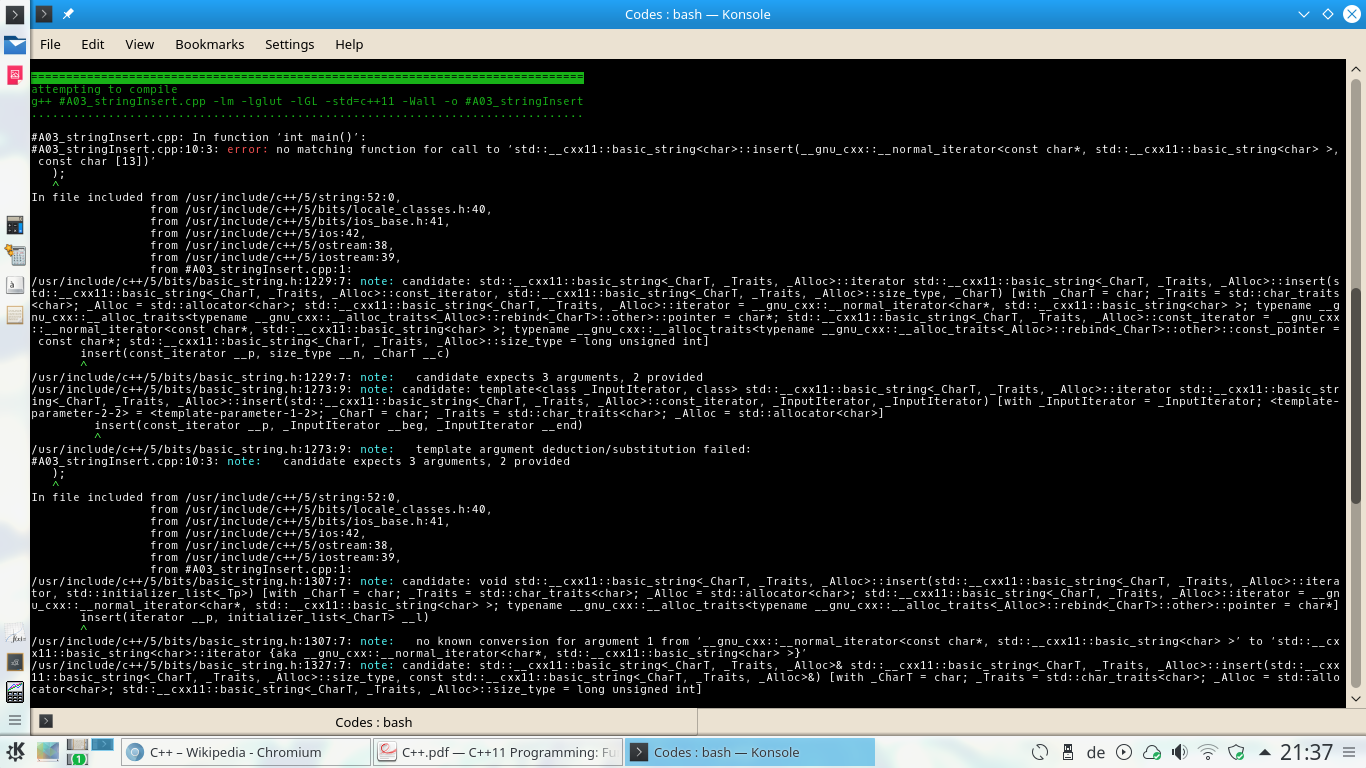
\includegraphics[width=.495\linewidth]{./gfx/cppFirst}
%
\vspace{-12pt}
\begin{itemize}
\item Bild: Fehlermeldung bei meinem ersten Kompilierdurchgang zu \emph{Insert Strings}.
\item Fehlermeldungen erstrecken sich über mehr als eine Bildschirmseite
\item Fehler war unnötige Referenz auf Startpunkt
\item[$\Rightarrow$] Erst wer C sicher beherrscht, wird C++ nutzen können
\end{itemize}
%
\end{frame}

% =========================================================================== %

\begin{frame}{Klassen -- Objektorientierung}
%
\begin{columns}[T]
\column{.5\linewidth}
\begin{itemize}
\item Weiterentwicklung von \mintinline{c}{structs}
\item Funktionen zu Klasse zugeordnet
\item Zugriff auf Records der Klasse über Schlüsselwort \mintinline{c++}{this}: Pointer auf Klassenobjekt
\item Constructors und Destructors
	\begin{itemize}
	\item Automatischer Funktionsaufruf beim Erstellen und oder Freigeben
	\item Betrifft auch Verlassen des Scopes
	\end{itemize}
% CTOR, DTOR
\end{itemize}
%
\column{.5\linewidth}
\begin{itemize}
\item Zugriffsbeschränkung: \mintinline{c++}{private} und \mintinline{c++}{public}
	\begin{itemize}
	\item \mintinline{c++}{public} -- Zugriff auf Record von überall -- wie aus C bekannt
	\item \mintinline{c++}{private} -- Zugriff nur von Klassenmethoden aus
	\item Sinn: Verhindere \enquote{unsinnige} Zustände (Bsp: Matrix-Klasse: Record Zeilen passt nicht 
		zum  Dateninhalt)
	\end{itemize}
\end{itemize}
\end{columns}
%
\end{frame}

% =========================================================================== %

\begin{frame}[fragile]
%
\tcbset{width=.495\linewidth, on line, height=7.8cm}
%
\begin{codebox}[Beispiel: Klasse in C++ ...]
\begin{minted}[fontsize=\scriptsize, linenos]{c++}
#include <iostream>
using namespace std;

class Mat {
private: // internal mechanisms
   int rows, cols;
   double * data;
   
public:  // exposed to the user
   int getRows();
   int getCols();
   double getElement(int row, int col);

   // constructors
   Mat ();
   Mat (int rows, int cols);

   // destructor
   ~Mat ();
};
\end{minted}
\end{codebox}
%	
\begin{codebox}[... Fortsetzung ...]
\begin{minted}[fontsize=\scriptsize, linenos, firstnumber=last]{c++}
Mat::Mat (int rows, int cols) {
   this->rows = rows;
   this->cols = cols;
   this->data = new double[rows * cols];
}
Mat::~Mat () {delete this->data;}

int Mat::getRows() {return this->rows;}
int Mat::getCols() {return this->cols;}

double Mat::getElement(int r, int c) {
   if (
      (r >= this->rows) || (r < 0) ||
      (c >= this->cols) || (c < 0)
   ) {
      return 0;
   } else {
      return this->data[r * cols + c];
   }
}
\end{minted}
\end{codebox}
%
\end{frame}

% =========================================================================== %

\begin{frame}[fragile]
%
\begin{columns}[T]
\column{.55\linewidth}
\vspace{-6pt}
\begin{codebox}[... Fortsetzung]
\begin{minted}[fontsize=\scriptsize, linenos, firstnumber=last]{c++}
int main () {
   Mat Empty;
   Mat ThreeByThree(3, 3);

   cout << Empty.getRows() << endl;
   cout << ThreeByThree.getRows() << endl;
   cout << ThreeByThree.getElement(1, 1);

   return 0;
}
\end{minted}
\end{codebox}
%
\begin{itemize}
\item Denkweise: \texttt{Objekt.Aktion(Parameter)}
\item Abgekapselte Systeme (Objekte) erlauben mehr Sicherheit, indem Wechselwirkungen beschränkt werden
\item \enquote{Semi-Globale Variablen} (\ie Records)
\end{itemize}
%	
\column{.45\linewidth}
\begin{itemize}
\item Zugriffskontrolle erhöht Anwendungssicherheit
\item Constructors: Objekt automatisch sinnvoll vorbereiten
\item Destructor: Zugriff auf Ressourcen freigeben
\item \mintinline{c++}{new} und \mintinline{c++}{delete}: Wie \mintinline{c++}{malloc} und 
	\mintinline{c++}{free}, aber rufen automatisch Constructors und Destructors auf
\item Overloaded Functions: Selber Name, unterschiedliche Parameterliste, unterschiedlicher Code.
\end{itemize}
\end{columns}
%
\end{frame}

% =========================================================================== %

\begin{frame}[fragile]{Templates}
%
\begin{columns}[T]
\column{.51\linewidth}
\begin{itemize}
\item Typen-unabhängige, abstrakte Formulierung von Routinen und Klassen
\item Klasse: Hier jeder beliebige Datentyp, also primitive Typen (z.\,B. \mintinline{c}{int}) bis hin zu
	Klassen wie zuvor kennen gelernt
\item Intern: Umsetzung ähnlich wie Makros: Präprozessor erstellt passenden Code
\item Template-Parameter: Klasse
\item Auch möglich: Template-Parameter Wert
	\begin{itemize}
	\item Erzeugt Funktion, in der Parameter \emph{hardcoded} auftaucht
	\item Manchmal dadurch Performance-Gewinn
	\end{itemize}
\end{itemize}
%
\column{.5\linewidth}
\vspace{-16pt}
\begin{codebox}[Beispiel: Templates]
\begin{minted}[fontsize=\scriptsize, linenos]{c++}
#include <iostream>
using namespace std;

template <class T>
T sum (T a, T b) {
    T result = a + b;
    return result;
}

int main () {
    int    i=5  , j=6  , k;
    double f=2.0, g=0.5, h;
    k = sum<int>   (i, j);
    h = sum<double>(f, g);
    cout << k << h << endl;
    return 0;
}
\end{minted}
\tiny \url{http://www.cplusplus.com/doc/tutorial/functions2/}
\vspace{-6pt}
\end{codebox}
\end{columns}
%
\end{frame}

% =========================================================================== %

\begin{frame}{Template-Klasse \texttt{vector}}
%
\begin{columns}[T]
\column{.5\linewidth}
\begin{itemize}
\item konsekutive Listen von Objekten gleichen Datentyps
\item \enquote{n-Tupel gleichen Datentyps} -- Liste von n Werten
\item Interface für dynamische C-Arrays
\item Methoden erlauben häufige Aufgaben (Vergrößern, Sortieren, ...) bequem \emph{und} effizient
\item Template: Für jeden beliebigen Datentyp machbar -- auch für eigene \texttt{struct}s oder Klassen.
\end{itemize}
%
\column{.5\linewidth}
\begin{itemize}
\item Methoden:
	\begin{itemize}
	\item \texttt{at}, \texttt{size}, \texttt{capacity} -- wie bei \texttt{string}
	\item \texttt{begin}, \texttt{end} -- erstes und letztes Element
	\item \texttt{clear}, \texttt{erase}, \texttt{swap}, \texttt{resize}
	\end{itemize}
\item Bereitgestellte Algorithmen
	\begin{itemize}
	\item \texttt{sort}
	\item \texttt{for\_each} -- Schleifen mit \texttt{vector}s
	\item \texttt{count\_if} -- Zählen mit Bedingung
	\end{itemize}
\item \url{http://en.cppreference.com/w/cpp/container/vector}
\end{itemize}
\end{columns}
%
\end{frame}

% =========================================================================== %

\begin{frame}[fragile]
%
\tcbset{width=.495\linewidth, on line, height=7.8cm}
%
\begin{codebox}[Beispiel: Vectors]
\begin{minted}[fontsize=\scriptsize, linenos]{c}
#include <iostream>
#include <vector>
 
void print_vec(
    const std::vector<int>& vec
) {
    for (auto x: vec) {
         std::cout << ' ' << x;
    }
    std::cout << '\n';
}
 
int main () {
    std::vector<int> vec(3,100);
    print_vec(vec);
 
    auto it = vec.begin();
    it = vec.insert(it, 200);
    print_vec(vec);
\end{minted}
\end{codebox}
%	
\begin{codebox}[Beispiel: ... Fortsetzung]
\begin{minted}[fontsize=\scriptsize, linenos, firstnumber=last]{c}
    vec.insert(it,2,300);
    print_vec(vec);
 
    // it no longer valid, get new one:
    it = vec.begin();
 
    std::vector<int> vec2(2,400);
    vec.insert(
        it+2, 
        vec2.begin(), 
        vec2.end()
    );
    print_vec(vec);
 
    int arr[] = { 501,502,503 };
    vec.insert(vec.begin(), arr, arr+3);
    print_vec(vec);
}
\end{minted}
\tiny \url{http://en.cppreference.com/w/cpp/container/vector/insert}
\end{codebox}
%
\end{frame}

% =========================================================================== %

\begin{frame}{Werbung}
%
\begin{tcolorbox}
Der Kurs \href{http://www.physik.uni-regensburg.de/studium/it/c++kurs}{\thus \emph{Programmieren mit C++ und der Qt-Klassenbibliothek} $\leftarrow$} liefert in 2 Wochen eine sehr gute, intensive Einführung in das Programmieren mit C++ und stellt außerdem die Bibliothek Qt vor.

\vspace{3pt}
In der ersten Woche wird aufbauend auf unsere Kenntnisse C++ erklärt und in Übungen angewandt. Die hier angerissenen Konzepte und vieles mehr werden in großer Detailtiefe behandelt und erlauben so erste Schritte (!) in C++.

\vspace{3pt}
Die zweite Woche zeigt die Klassenbibliothek Qt, die verhältnismäßig einfach erlaubt, ansprechende \emph{graphische} Userinterfaces (GUIs) zu erstellen.
\end{tcolorbox}
%
\end{frame}